\documentclass[singlespacing,12pt,parskip,headsepline,consistentlayout]{article}
\usepackage{float}
\usepackage{caption}
\usepackage{biblatex}

\usepackage{ragged2e}
\usepackage{listings}
\usepackage[skip=10pt plus1pt, indent=40pt]{parskip}
\renewcommand{\familydefault}{\sfdefault}
\usepackage{graphicx}
\graphicspath{ {./img/} }
\usepackage[utf8]{inputenc}
\usepackage{indentfirst}
\usepackage[main=english,polish]{babel}
\addbibresource{ref.bib}
\usepackage{xcolor}
\usepackage{fontspec}
\setsansfont{Arial}
\definecolor{codegreen}{rgb}{0,0.6,0}
\definecolor{codegray}{rgb}{0.5,0.5,0.5}
\definecolor{codepurple}{rgb}{0.58,0,0.82}
\definecolor{backcolour}{rgb}{0.97,0.97,0.97}

\lstdefinestyle{mystyle}{
    backgroundcolor=\color{backcolour},   
    commentstyle=\color{codegreen},
    keywordstyle=\color{magenta},
    numberstyle=\tiny\color{codegray},
    stringstyle=\color{codepurple},
    basicstyle=\helvet\footnotesize,
    breakatwhitespace=false,         
    breaklines=true,                 
    captionpos=b,                    
    keepspaces=true,                 
    numbers=left,                    
    numbersep=5pt,                  
    showspaces=false,                
    showstringspaces=false,
    showtabs=false,                  
    tabsize=2
}
\lstset{style=mystyle}
\date{}

\begin{document}

\begin{titlepage}
\begin{center}
    


\includegraphics{pjatk_icon.png}
\vspace{1cm}
{\bfseries Wydział Informatyki}

\vspace{1cm}
{\bfseries Katedra Baz Danych}

{Specjalizacja Baz Danych}

\vspace{3cm}
{\bfseries Tu Alexander, Zembrzuska Magdalena, Zviezdin Illia}

{numery albumów: s20290, s20983, s21120}

\vspace{2cm}

{\bfseries Stworzenie narzędzia do edukacji studentów kierunków medycznych za pomocą symulacji badań EKG }

\vspace{2cm}
\end{center}
\begin{flushright}
{Praca inżynierska}

{dr Ida Jokisz}    
\end{flushright}


\vfill
\begin{center}
{Warsaw, styczeń  2022}    
\end{center}


\end{titlepage}
\pagebreak

\begin{titlepage}
\begin{center}
    {\large\bfseries Streszczenie}
\end{center}




{Głównym celem pracy jest stworzenie funkcjonalnej i intuicyjnej aplikacji internetowej, która ma pomóc w kształceniu studentów kierunków medycznych na polskich uczelniach oraz dać profesorom narzędzie to łatwego sprawdzenia wiedzy w zakresie analizy wykresów elektrokardiogramów i na tej podstawie oceny zdrowia pacjenta, a także zdiagnozowania przebytych chorób czy zmian morfologicznych.}

\vspace{1cm}

{Praca zawiera szczegółowy opis funkcjonalności dostarczanych przez web-aplikację, architekturę projektu, sposób w jaki różne części projektu są ze sobą związane, modele zapewniające wizualizacje pewnych konceptów, oprogramowanie użyte do budowy aplikacji wraz z uzasadnieniem wyboru danego oprogramowania oraz instrukcje użytkowania web-aplikacji wraz z testami.}
\vfill
\noindent{\bfseries Słowa kluczowe}: elektrokardiogram, aplikacja internetowa, aplikacja fullstack, aplikacja medyczna, aplikacja szkoleniowa
\end{titlepage}


\begin{titlepage}
\centering
\begin{center}

\includegraphics{pjatk_icon.png}
\vspace{1cm}
{\bfseries Faculty of Information Technology}

\vspace{1cm}
{\bfseries Chair of Databases}

{Databases Specialization}

\vspace{3cm}
{\bfseries Tu Alexander, Zembrzuska Magdalena, Zviezdin Illia}

{student no.: s20290, s20983, s21120}

\vspace{2cm}

{\bfseries Creation of a tool for education of students of medical related studies with simulating ECG}

\vspace{2cm}    
\end{center}

\begin{flushright}
{Bachelor of Engineering Thesis}

{dr Ida Jokisz}
\end{flushright}

\vfill
\begin{center}
{Warsaw, January 2022 }    
\end{center}

\end{titlepage}
\pagebreak
\begin{titlepage}
\begin{center}
    {\large\bfseries Abstract}
\end{center}

{The main objective of the project was to develop a convenient, accessible and simple to use web-application to assist professors to teach medical students how to recognize certain electrocardiogram (ECG) diagrams. The aim of this web-application is to create an educational platform with highly specialized questions designed to test and teach medical students.}
\vspace{1cm}

{The paper contains a detailed description of the functionalities provided by the web-application, the architecture of the project, how each part of the project works in combination with another part, models that provide visual representations, softwares used to build the application including the reasons for the choice of a certain software and manuals for using the web-application along with the testings.}

\vfill
\noindent{\bfseries Keywords}: electrocardiogram, web-application, fullstack application, medical application, training application
\end{titlepage}

\pagebreak
\tableofcontents
\pagebreak
\listoffigures
\listoftables
\pagebreak

\begin{titlepage}
\begin{center}
    {\large\bfseries Abbreviations and Acronyms}
\end{center}


\begin{center}
    \begin{tabular}{ |p{1.75cm}|p{4.5cm}|  |p{1.75cm}|p{4.5cm}|}
    \hline
 ECG & Electrocardiogram & JS & Javascript \\
 \hline
 TS & Typescript & SPA & Single Page Application \\
 \hline

 API & Application programming interface &  D3 & Data-Driven Documents \\
 
 \hline
 SQL & Structured Query Language & OAuth & Open Authorization \\
 
 \hline
 C4 & context, containers, components, and code & C\# & Csharp \\
 \hline
 
 URL & Uniform Resource Locator & DOM & Document Object Model \\
 \hline
  ASP.NET & Active Server Pages Network Enabled Technologies & CRUD & CREATE, READ, UPDATE and DELETE\\
\hline
ORM & Object-relational mapping & UML & Unified Modeling Language\\
\hline
REST & representational state transfer & JSON & JavaScript Object Notation\\
\hline
JWT & JSON Web Token & IOC & Inversion of Control \\
\hline
HTTP & Hypertext Transfer Protocol & SMTP & Simple Mail Transfer Protocol\\
\hline
\end{tabular}
\end{center}
\end{titlepage}


\pagebreak
\section{Introduction}
The purpose of this document is to provide a thorough overview of the methods and tools used to create the application, as well as the architectural philosophies that guided its development. It will include descriptions of the various functionalities of the system and diagrams illustrating the various processes within the application. The goal is to give a comprehensive understanding of how the application operates and the reasoning behind its design.

One of the main objectives of this document is to detail the different technologies and frameworks that were utilized in the creation of the application. This will include programming languages, libraries, and any other tools that were integral to the development process. Additionally, the document will delve into the various architectural patterns and principles that were followed, such as modularity, separation of concerns, and scalability.

Overall, this document aims to provide a comprehensive understanding of the inner workings of the application and the thought process behind its design. By presenting a clear and detailed explanation of the methods and tools used, as well as the architectural philosophies that guided the development, it is hoped that this document will serve as a valuable resource for anyone looking to gain a deeper understanding of the application.


\subsection{Aims and objectives}

The aim of this educational application is to provide a platform for simulating electrocardiograms, which are graphical representations of the electrical activity of the heart. This application is specifically designed for professors to use as a means of testing their students' knowledge of electrocardiograms, as well as for students to use as a tool for practicing and reinforcing their understanding of these important medical records.

By using this application, professors will have a way to assess their students' knowledge and skills in interpreting electrocardiograms, which are vital for diagnosing and treating a wide range of heart conditions. Students, on the other hand, will be able to practice recognizing patterns in electrocardiograms and identifying the diseases that can cause them. This will not only help them to better understand this complex subject matter, but it will also prepare them for the real-world challenges they will face as healthcare professionals.

Overall, the purpose of this application is to assist in the education and training of students in the field of electrocardiography, enabling them to become proficient in recognizing and interpreting electrocardiograms. By providing a simulated environment for practicing and learning, this application aims to help students develop the knowledge and skills they need to succeed in their careers and make a positive impact in the lives of their patients.


\subsection{Scope}

This is the second subsection
As an educational platform, it is crucial that this application is designed in a way that allows users to easily access and utilize all of its functionalities. To achieve this, we have focused on creating a simple and intuitive interface for our users.

One of the key features of this application is the ability to visualize electrocardiograms, which are graphical representations of the electrical activity of the heart. These are an essential part of the application, as they provide the basis for learning and practice in interpreting these important medical records. To ensure that our visualizations are as accurate and realistic as possible, we have chosen to use actual electrocardiogram images as the basis for our visualizations. This means that the visualizations are based on real case scenarios, providing a highly accurate representation of what users can expect to encounter in their professional careers.

Overall, the scope of this application is to provide an educational platform for professors and students to learn about and practice interpreting electrocardiograms. By using real electrocardiogram images as the basis for our visualizations, we aim to provide a valuable and realistic tool for those seeking to improve their knowledge and skills in this field.

\section{Functional requirements}

The functional requirements of the application are the specific tasks and functions that it is intended to perform. These requirements serve as the foundation for the design and development of the application, and must be carefully considered in order to ensure that the application meets the needs of its users.

In order to clearly understand the functional requirements of the application, it is necessary to consider the various factors that may affect its performance. These factors may include the intended user base, the operating environment, and any external systems or services that the application may need to interact with. Additionally, it is important to consider the various scenarios that the application may encounter, as this will help to identify any potential challenges or issues that may arise during its operation.

Once the functional requirements of the application have been identified, the next step is to design and develop the application in a way that meets these requirements. This may involve choosing specific programming tools and frameworks, designing the backend and frontend of the application, and creating an architecture for the database. It is also important to carefully test the application and ensure that it functions correctly in all scenarios, and to carefully plan the deployment process in order to ensure a smooth transition to live operation.

Overall, the functional requirements of the application are a crucial factor in its design and development, and must be carefully considered in order to ensure that the application meets the needs of its users and operates smoothly in all scenarios.

\subsection{Description of the system functionalities}

The application is designed to offer a range of functionalities to its users. These functionalities include basic features such as user authentication and authorization, as well as more specialized features that are specific to the intended use of the application.

\pagebreak

\begin{center}    
\captionof{table}{Actors}\label{tbl:actors}
\begin{tabular}{ |p{1cm}|p{3cm}|p{9cm}|  }
\hline

\multicolumn{3}{|c|}{\bf{Actors}} \\
\hline
\bf{ID}& \bf{Name}&\bf{Description} \\
\hline
1&Professor&Professors have administrative access to students and can assign tasks\\
\hline
2&Students&Students have basic access to functionalities \\
2&Pseudo Admin&Pseudo admin has minimum administrative access to all users\\
\hline
\end{tabular}

\pagebreak
\captionof{table}{Functionalities}\label{tbl:functionalities}
\begin{tabular}{ |p{1cm}|p{3cm}|p{9cm}|  }
\hline

\multicolumn{3}{|c|}{\bf{Functionalities}} \\
\hline
\bf{ID}& \bf{Functionality}&\bf{Description} \\
\hline
1&Login&The system will check the given credentials during login and allow users to access the app given the correct info.\\
\hline
2&Register&The system sends a confirmation email when a new account is registered. \\
\hline
3&Logout&Users can logout\\
\hline
4&Create group&A new group will be created based on the doctor’s request when creating the group and a unique group code for that group will be generated upon creation.\\
\hline
5&Assign task&The assign task functionality will allow doctors to assign tasks to chosen groups.\\
\hline
6&Activate account&Users will be able to activate account which they have registered.\\
\hline
7&Start a task&Users will be able to access the tasks assigned to them and start solving them.\\
\hline
8&Reset password&Users will be able to reset password if they lost their credentials.\\
\hline
9&Remove a group&Professors will be able to remove groups which they have created.\\
\hline
10&Remove user from group&Professors will be able to remove users that are in the group they created.\\
\hline
11&Remove task from group&Professors will be able to remove tasks they have assigned to their groups.\\
\hline
12&Regenerate group code&Professors will be able to regenerate group code of their groups.\\
\hline
13&Join a group&Users will be able to join a group given corresponding group code.\\
14&Update role&Pseudo admin has permission to update user's role.\\
\hline
\end{tabular}

\end{center}


\subsection{Use case diagram}
\begin{figure}[H]
    \centering
    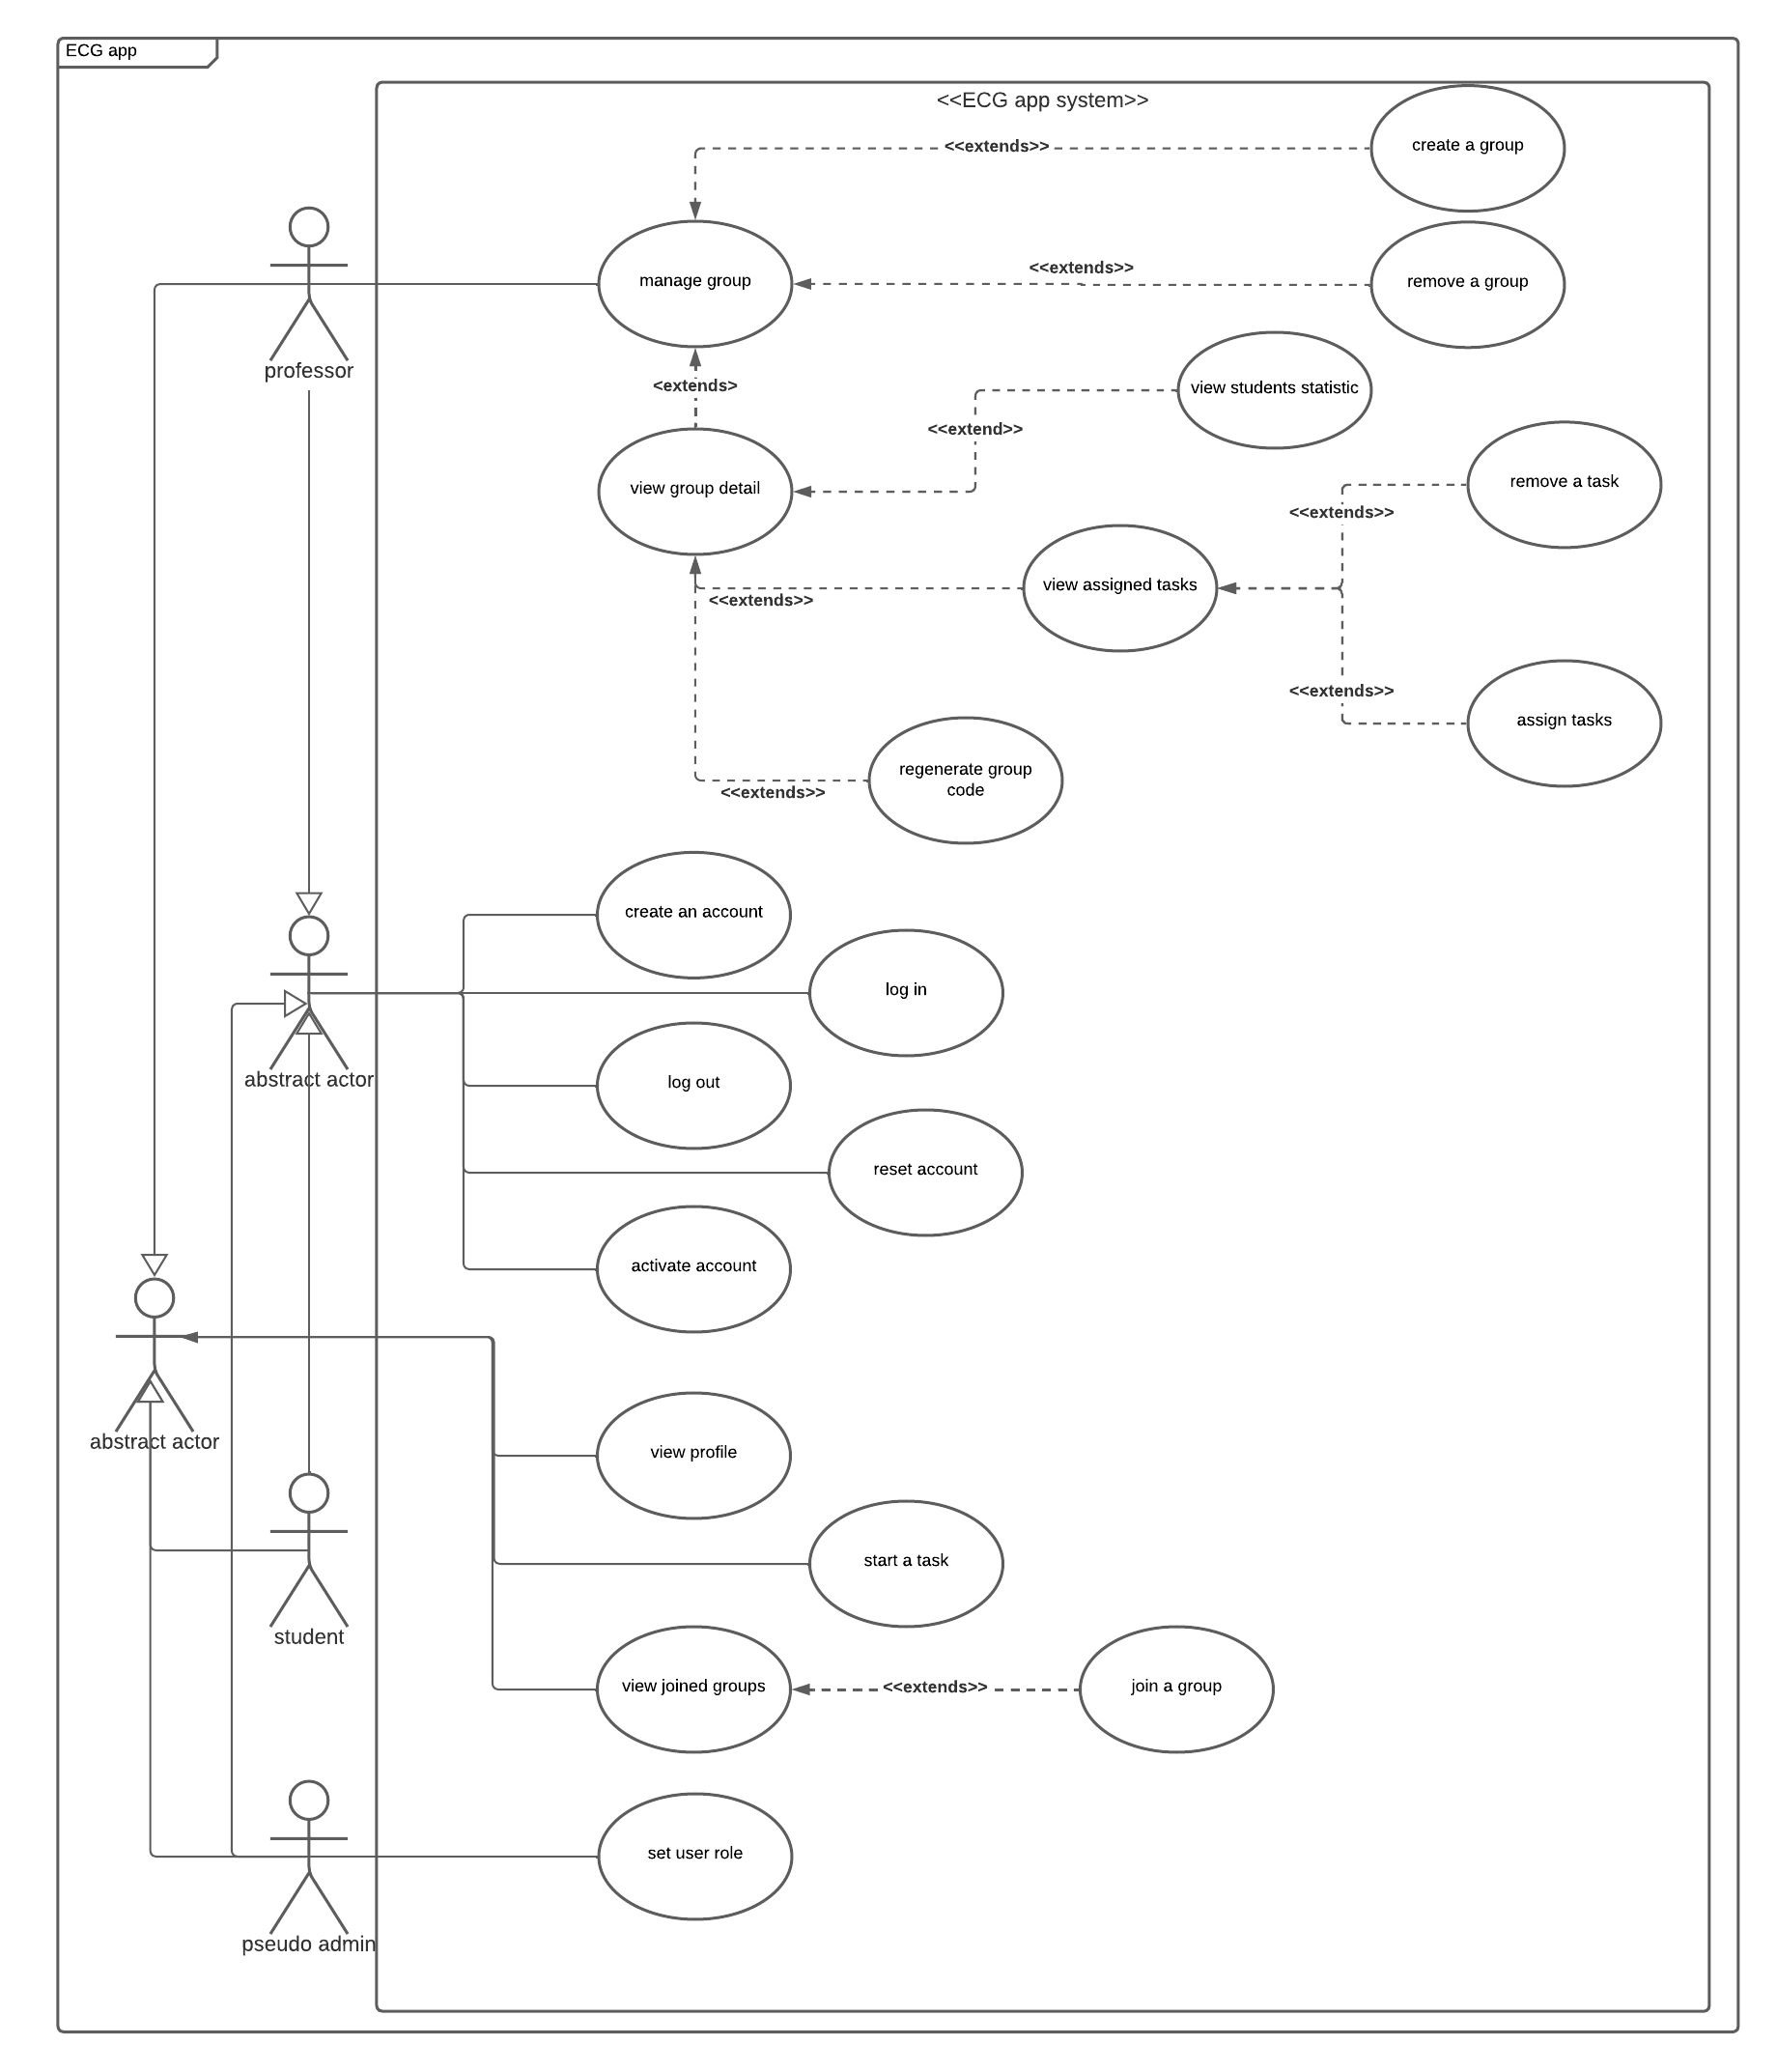
\includegraphics[width=\textwidth,height=\textheight,keepaspectratio]{img/PRO - diagrams.png}
    \caption{Use case diagram}
\end{figure}


\pagebreak

\subsection{Entity diagram}
\begin{figure}[H]
    \centering
    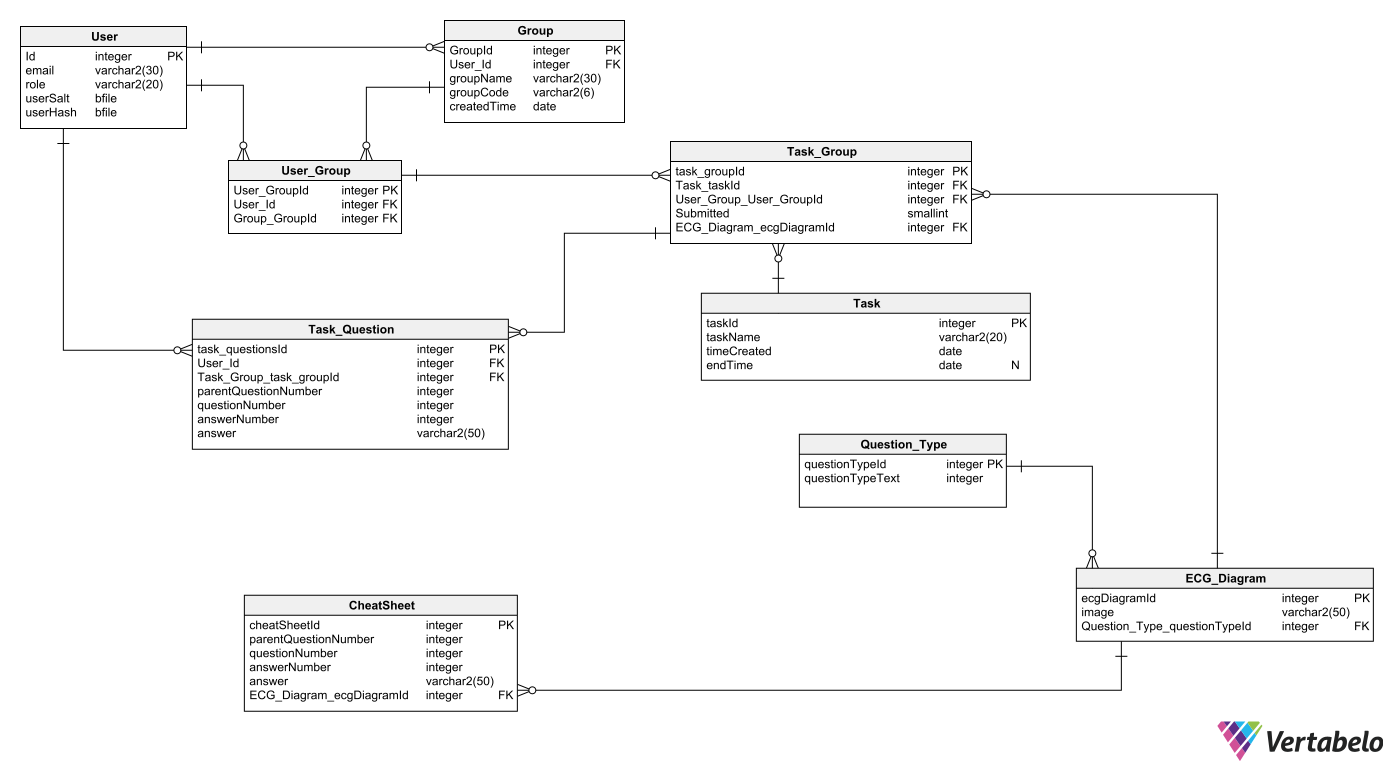
\includegraphics[width=\textwidth,height=\textheight,keepaspectratio]{img/project_database-2023-01-06_14-26.png}
    \caption{Entity diagram}
\end{figure}
\pagebreak
\subsection{Use case scenarios}

\subsubsection{Use case 1 - Log in}
\begin{flushleft}

\vspace{0.2cm}
\hline
\vspace{0.2cm}
{\bfseries Title}: {Log in}

{\bfseries Description}: {A student or professor can be authorized into service and authenticated based on provided credentials}

{\bfseries Primary Actors}: {Student, Professor}

{\bfseries Preconditions}: The user is a valid and verified person who has access to the system

{\bfseries Postconditions}: {The user is directed to the landing page after login}

{\bfseries Main Success Scenario}

\begin{enumerate}
      \item The user clicks the {\bfseries Login} button
  \item A credential form is displayed
  \item The user enters credential
  \item The system checks the validity of credentials
  \item The landing page after login is displayed
\end{enumerate}
 
{\bfseries Extensions}

\begin{enumerate}
  \item No valid credentials have been entered
  \begin{enumerate}
      \item System informs the user of invalid credential
      \item Flow returns to step 2 of basic flow
  \end{enumerate}
\end{enumerate}

{\bfseries Frequency of use}: very frequent

{\bfseries Priority}: high

\end{flushleft}

\pagebreak
\subsubsection{Use case 2 - Register}
\begin{flushleft}
\vspace{0.2cm}
\noalign \hline
\vspace{0.2cm}
{\bfseries Title}: {Register}

{\bfseries Description}: {A user is allowed to register an account using an email belonging to the school’s domain.}

{\bfseries Primary Actors}: {Abstract User}

{\bfseries Preconditions}: The user is a valid and verified person who has access to the system.

{\bfseries Postconditions}: {The user is granted login permission by the system.}

{\bfseries Main Success Scenario}

\begin{enumerate}
      \item The user clicks the {\bfseries Register} button
      \item The app redirects the user to the registration page with form
      \item The user enters their email and password for registration
      \item The system sends a validation email to the user’s email address
      \item The system grants login permission to the corresponding account once validation is completed
\end{enumerate}
 
{\bfseries Extensions}

\begin{enumerate}
  \item The user enters an email not belonging to the school’s domain
  \begin{enumerate}
      \item The system informs the user of the wrong domain
      \item Flow returns to Step 3 of main scenario
  \end{enumerate}
  \item The user does not verify the email
\end{enumerate}

{\bfseries Frequency of use}: often

{\bfseries Priority}: high

\end{flushleft}

\pagebreak
\subsubsection{Use case 3 - Log out}
\begin{flushleft}
\vspace{0.2cm}
\hline
\vspace{0.2cm}
{\bfseries Title}: {Log out}

{\bfseries Description}: {A student or professor can log out of the web application when they need to}

{\bfseries Primary Actors}: {Professor, Student}

{\bfseries Preconditions}: The user is a valid and verified person who has access to the system and is already logged in.

{\bfseries Postconditions}: {The user is logged out from the web application.}

{\bfseries Main Success Scenario}

\begin{enumerate}
      \item The user clicks the {\bfseries Log out} button
      \item The system logs the user’s account out
      \item The user is taken to the main login page
\end{enumerate}
 
{\bfseries Extensions}

\begin{enumerate}
  \item The user is already logged out
  \begin{enumerate}
      \item The user is shown a successful logout interface
  \end{enumerate}
\end{enumerate}

{\bfseries Frequency of use}: often

{\bfseries Priority}: high

\end{flushleft}

\pagebreak
\subsubsection{Use case 4 - Create a group}
\begin{flushleft}
\vspace{0.2cm}
\hline
\vspace{0.2cm}
{\bfseries Title}: {Create a group}

{\bfseries Description}: {Allow professors to create groups for other users to join}

{\bfseries Primary Actors}: {Professor}

{\bfseries Preconditions}: The user is a valid and verified person who has access to the system and is already logged in

{\bfseries Postconditions}: {A new group is created}

{\bfseries Main Success Scenario}

\begin{enumerate}
      \item The user selects {\bfseries Create Group} in the {\bfseries Group Mangement} page
      \item The system verifies the user’s permission
      \item The user is shown a form to enter the name of group
      \item The user confirms the creation of group
      \item The system generates a unique 6-character long code for the group
\end{enumerate}
 
{\bfseries Extensions}

\begin{enumerate}
  \item The user does not have permission to create group
  \begin{enumerate}
      \item System does not create group
  \end{enumerate}
\end{enumerate}

{\bfseries Frequency of use}: often

{\bfseries Priority}: medium

\end{flushleft}

\pagebreak
\subsubsection{Use case 5 - Assign Task}
\begin{flushleft}
\vspace{0.2cm}
\hline
\vspace{0.2cm}
{\bfseries Title}: {Assign task}

{\bfseries Description}: {The assign task functionality will allow doctors to assign tasks to chosen groups.}

{\bfseries Primary Actors}: {Professor}

{\bfseries Preconditions}: The user is a valid and verified person who has access to the system and is already logged in

{\bfseries Postconditions}: {New task is assigned to the corresponding group}

{\bfseries Main Success Scenario}

\begin{enumerate}
      \item The user selects the desired topic and enters task name to assign to the chosen group
      \item The system verifies user’s permission
      \item The system creates new task for the group
      \item The page informs user of successful completion
\end{enumerate}
 
{\bfseries Extensions}

\begin{enumerate}
  \item User does not have permission to assign task
  \begin{enumerate}
      \item System does not create new task
  \end{enumerate}
\end{enumerate}

{\bfseries Frequency of use}: often

{\bfseries Priority}: high

\end{flushleft}

\pagebreak
\subsubsection{Use case 6 - Activate account}
\begin{flushleft}
\vspace{0.2cm}
\hline
\vspace{0.2cm}
{\bfseries Title}: {Activate account}

{\bfseries Description}: {Users will be able to activate account which they have registered}

{\bfseries Primary Actors}: {Professor, Student}

{\bfseries Preconditions}: The user is a valid and verified person who has access to the system

{\bfseries Postconditions}: {The account is activated}

{\bfseries Main Success Scenario}

\begin{enumerate}
      \item The user accesses the url that holds activation token provided in the email
      \item The system accepts the requests and checks if the activation token is valid
      \item The system activates the account
      \item The page informs user of successful activation
\end{enumerate}
 
{\bfseries Extensions}

\begin{enumerate}
  \item The activation token is invalid
  \begin{enumerate}
      \item The system does not proceed with the request
  \end{enumerate}
  \item The account is already activated
  \begin{enumerate}
      \item The system does not proceed with the request
  \end{enumerate}
\end{enumerate}

{\bfseries Frequency of use}: often

{\bfseries Priority}: high

\end{flushleft}

\pagebreak
\subsubsection{Use case 7 - Start a task}
\begin{flushleft}
\vspace{0.2cm}
\hline
\vspace{0.2cm}
{\bfseries Title}: {Start a task}

{\bfseries Description}: {Users will be able to access the tasks assigned to them and start solving them}

{\bfseries Primary Actors}: {Professor, Student}

{\bfseries Preconditions}: The user is a valid and verified person who has access to the system

{\bfseries Postconditions}: {The chosen task is displayed}

{\bfseries Main Success Scenario}

\begin{enumerate}
      \item The user selects a task to start
      \item The system takes user to the task page
\end{enumerate}
 
{\bfseries Extensions}

\begin{enumerate}
  \item The user is not verified
  \begin{enumerate}
      \item The system does not proceed with the request
  \end{enumerate}
\end{enumerate}

{\bfseries Frequency of use}: often

{\bfseries Priority}: high

\end{flushleft}

\pagebreak
\subsubsection{Use case 8 - Reset password}
\begin{flushleft}
\vspace{0.2cm}
\hline
\vspace{0.2cm}
{\bfseries Title}: {Reset password}

{\bfseries Description}: {Users will be able to reset password if they lost their credentials}

{\bfseries Primary Actors}: {Professor, Student}

{\bfseries Preconditions}: The user is a valid and verified person who has access to the system

{\bfseries Postconditions}: {The password is reset}

{\bfseries Main Success Scenario}

\begin{enumerate}
      \item The user enters the page to reset password
      \item The user enters the corresponding email address
      \item The system checks if email exists
      \item The system send url with password token to the given email address
      \item The user accesses the given url provided in the email
      \item The page shows a form for the user to enter desired new password
      \item The user submits the reset request
      \item The system checks if request is valid
      \item The system resets the password
      \item The page informs user of successful reset
\end{enumerate}
 
{\bfseries Extensions}

\begin{enumerate}
  \item The email does not exist
  \begin{enumerate}
      \item The system does not proceed with the request
  \end{enumerate}
  \item The password token is not valid
  \begin{enumerate}
      \item The system does not proceed with the request
  \end{enumerate}
\end{enumerate}

{\bfseries Frequency of use}: often

{\bfseries Priority}: high

\end{flushleft}

\pagebreak
\subsubsection{Use case 9 - Remove a group}
\begin{flushleft}
\vspace{0.2cm}
\hline
\vspace{0.2cm}
{\bfseries Title}: {Remove a group}

{\bfseries Description}: {Professors are authorized to remove groups created by them}

{\bfseries Primary Actors}: {Professor}

{\bfseries Preconditions}: The user is a valid and verified person who has access to the system and is already logged in

{\bfseries Postconditions}: {Group is removed}

{\bfseries Main Success Scenario}

\begin{enumerate}
      \item The user selects {\bfseries Remove} button of the desired group
      \item The system verifies user’s permission
      \item The system removes the group
      \item The page shows a success message to notify the user
\end{enumerate}
 
{\bfseries Extensions}

\begin{enumerate}
  \item The user does not have permission to remove the group
  \begin{enumerate}
      \item System does not remove group
  \end{enumerate}
\end{enumerate}

{\bfseries Frequency of use}: rarely

{\bfseries Priority}: low

\end{flushleft}

\pagebreak
\subsubsection{Use case 10 - Remove user from group}
\begin{flushleft}
\vspace{0.2cm}
\hline
\vspace{0.2cm}
{\bfseries Title}: {Remove user from group}

{\bfseries Description}: {Professors will be able to remove users that are in the group they created}

{\bfseries Primary Actors}: {Professor}

{\bfseries Preconditions}: The user is a valid and verified person who has access to the system

{\bfseries Postconditions}: {The user is removed from the group}

{\bfseries Main Success Scenario}

\begin{enumerate}
      \item The user clicks on the {\bfseries Remove} button for the chosen user
      \item The system checks if the user has permission
      \item The system removes the selected user from the group
      \item The page updates the list
\end{enumerate}
 
{\bfseries Extensions}

\begin{enumerate}
  \item The user does not have permission
  \begin{enumerate}
      \item The system does not proceed with request
  \end{enumerate}
\end{enumerate}

{\bfseries Frequency of use}: rarely

{\bfseries Priority}: low

\end{flushleft}

\pagebreak
\subsubsection{Use case 11 - Remove task from group}
\begin{flushleft}
\vspace{0.2cm}
\hline
\vspace{0.2cm}
{\bfseries Title}: {Remove task from group}

{\bfseries Description}: {Professors will be able to remove tasks they have assigned to their groups}

{\bfseries Primary Actors}: {Professor}

{\bfseries Preconditions}: The user is a valid and verified person who has access to the system

{\bfseries Postconditions}: {The chosen task is removed from the group}

{\bfseries Main Success Scenario}

\begin{enumerate}
      \item The user clicks on {\bfseries Remove} button on the desired task
      \item The system checks if the user has permission
      \item The system removes task from the group
      \item The page updates the list
\end{enumerate}
 
{\bfseries Extensions}

\begin{enumerate}
  \item The user does not have permission to remove task
  \begin{enumerate}
      \item The system does not carry out the request
  \end{enumerate}
\end{enumerate}

{\bfseries Frequency of use}: rarely

{\bfseries Priority}: medium

\end{flushleft}

\pagebreak
\subsubsection{Use case 12 - Regenerate group code}
\begin{flushleft}
\vspace{0.2cm}
\hline
\vspace{0.2cm}
{\bfseries Title}: {Regenerate group code}

{\bfseries Description}: {Professors will be able to regenerate group code of their groups}

{\bfseries Primary Actors}: {Professor}

{\bfseries Preconditions}: The user is a valid and verified person who has access to the system

{\bfseries Postconditions}: {The group code for the group is regenerated}

{\bfseries Main Success Scenario}

\begin{enumerate}
      \item The user clicks on the {\bfseries Regenerate code} button
      \item The system checks if the user has permission
      \item The system regenerates group code
      \item The page updates the group code
\end{enumerate}
 
{\bfseries Extensions}

\begin{enumerate}
  \item The user does not have permission
  \begin{enumerate}
      \item The system does not proceed with request
  \end{enumerate}
\end{enumerate}

{\bfseries Frequency of use}: rarely

{\bfseries Priority}: medium

\end{flushleft}

\pagebreak
\subsubsection{Use case 13 - Join a group}
\begin{flushleft}
\vspace{0.2cm}
\hline
\vspace{0.2cm}
{\bfseries Title}: {Join a group}

{\bfseries Description}: {Users will be able to join a group given corresponding group code}

{\bfseries Primary Actors}: {Professor, Student}

{\bfseries Preconditions}: The user is a valid and verified person who has access to the system

{\bfseries Postconditions}: {The user joins the group}

{\bfseries Main Success Scenario}

\begin{enumerate}
      \item The user enters the group code and submits request
      \item The system checks if request is valid
      \item The system adds the user to the group with corresponding group code
      \item The page updates the list
\end{enumerate}
 
{\bfseries Extensions}

\begin{enumerate}
  \item The request is not valid
  \begin{enumerate}
      \item The system does not proceed with request
  \end{enumerate}
  \item The user is already in the group
  \begin{enumerate}
      \item The system does not proceed with request
  \end{enumerate}
\end{enumerate}

{\bfseries Frequency of use}: rarely

{\bfseries Priority}: medium

\end{flushleft}

\pagebreak

\subsubsection{Use case 14 - Update role}
\begin{flushleft}
\vspace{0.2cm}
\hline
\vspace{0.2cm}
{\bfseries Title}: {Update role}

{\bfseries Description}: {Pseudo admin will be able to update users' role}

{\bfseries Primary Actors}: {Pseudo admin}

{\bfseries Preconditions}: The user is a valid and verified person who has access to the system

{\bfseries Postconditions}: {The user chosen by the pseudo admin will have role updated.}

{\bfseries Main Success Scenario}

\begin{enumerate}
      \item The user enters the desired email address and role
      \item The user submits the request
      \item The system checks if user has permission
      \item The system updates the role
      \item The system notifies user of successful update
\end{enumerate}
 
{\bfseries Extensions}

\begin{enumerate}
  \item The request is not valid
  \begin{enumerate}
      \item The system does not proceed with request
  \end{enumerate}
  \item The email address does not exist
  \begin{enumerate}
      \item The system does not proceed with request
  \end{enumerate}
\end{enumerate}

{\bfseries Frequency of use}: often

{\bfseries Priority}: high

\end{flushleft}

\section{Non-functional requirements}
\subsection{Usability}

It is crucial that the medical application is designed with usability in mind, as it will be used by a variety of non-technical users. This means that all features and functionality should be easily accessible and intuitive to use.

To achieve this, the app should have a coherent and logical layout, with clear and concise instructions for each feature. This will help medical students quickly and easily navigate to the resources and information they need, without being bogged down by the complexities of the technology.

Additionally, the app should be user-friendly and straightforward to use, so that medical students can focus on their studies rather than struggling with the app itself. By prioritizing usability, the app can be a valuable tool for medical students, helping them to efficiently access the resources and information they need to succeed in their studies.

\subsection{Security}

Ensuring the security of an application is a complex task that requires constant vigilance and attention. Despite our best efforts, it is possible that there may be overlooked issues or vulnerabilities that could compromise the security of the system. In the case of an internal application intended for use by a university, it is important to take extra precautions to ensure the safety of sensitive information and data.

One key factor to consider is that the application will be standalone, meaning that it will not be connected to any external systems or networks. This can significantly reduce the potential for a secondary breach, as there will be no link to other servers or databases. However, it is still important to take steps to secure the application itself, such as implementing strong passwords, enabling two-factor authentication, and regularly updating the system to fix any identified vulnerabilities.

In addition to technical measures, it is also important to consider the role of user education in maintaining the security of the application. By providing training and resources to users on how to protect their passwords and use the system responsibly, it is possible to significantly reduce the risk of a security breach.

The usage of OAuth for authentication and permission is another step made to improve the security of the application. \cite{oauthDocs} Users can securely authorize access to their data and resources, such as user profiles and server resources, using the open standard known as OAuth, without disclosing their login information. Since it enables users to log in using their university credentials and lowers the likelihood of password-related security breaches, this can be very helpful for an internal application. Additionally, because users don't need to remember numerous sets of login credentials, OAuth can offer a more smooth and user-friendly experience.

\section{Description of the prototypes}

The prototypes that are being developed are expected to possess a variety of features and capabilities. These include the ability to perform various functions, such as those that have been previously mentioned. It is important that the prototypes are able to fulfill all of the requirements and specifications that have been outlined in order to be deemed successful and effective. Therefore, it is essential that they are thoroughly tested and evaluated to ensure that they possess the necessary functionality to meet the intended goals and objectives.

\section{General description of the architecture}

The application will be composed of React Typescript for the frontend, C# for the backend and MySql for the database.

\section{C4 Model}

When you ask someone in the construction business to describe a building's design visually, they will likely show you site plans, floor plans, elevation views, cross-section views, and detail drawings. Comparatively, if you ask a software developer to represent the software architecture of a software system using diagrams, you'll probably end up with a muddled mess of boxes and lines... inconsistent notation (colour coding, shapes, line styles, etc.), ambiguous naming, unlabeled relationships, generic terminology, missing technology choices, mixed abstractions, etc. \cite{c4modelDocs}

The statement above has never been more true. From the perspective of a software developer, it is often very hard to communicate visually about how a certain software works, sometimes the visual representation given is too in depth or too vague, making things more complicated than it needs to be.

While Unified Modeling Language (UML), ArchiMate and SysML do exist \cite{c4modelDocs} as a form of visual communication between software developer and recipients, it is still lackluster in delivering the idea as it is simply too complex. An alternative to the previously mentioned ideas is the C4 model.

The C4 model provides an "abstraction-first" approach to diagramming softwares architecture, based on how software architects and developers think about and create software. The C4 model emphasises on simplicity for it to be easy to pick up. Furthermore, the C4 model is divide into 4 levels, not all of them must be used, only those that are important to deliver the idea. \cite{c4modelDocs}

In the following section, there are two levels of C4 model presented, level 1 and level 2, both of which will provide a visual concept of the architecture of the application, as well as explanation of the diagrams in question.

\subsection{Level 1}

\begin{figure}[H]
    \centering
    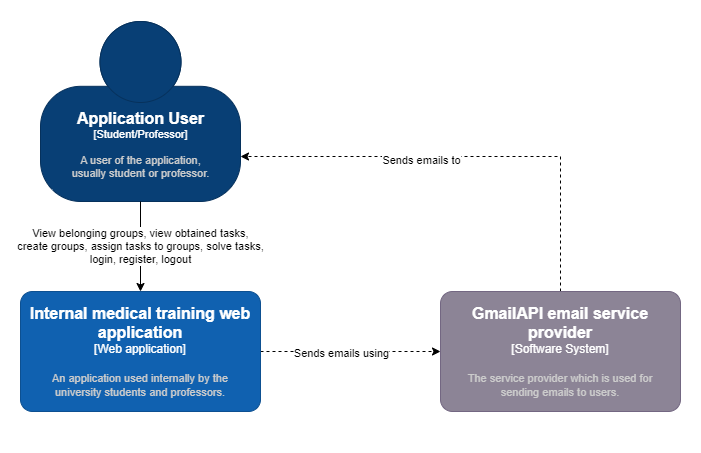
\includegraphics[width=\textwidth,height=\textheight,keepaspectratio]{img/c4_level1.png}
    \caption{Level 1 C4 model}
\end{figure}

In the level 1 C4 model shown, the system consists of three main components: the application users, the web application, and the email service provider. The application users are students and professors who interact with the web application to perform various tasks. These tasks include viewing the groups they belong to, viewing the tasks they are assigned, joining groups, registering, changing their password, logging in and out, and more.

The web application is responsible for managing the interactions between the application users and the email service provider. It provides the interface through which the application users can perform these tasks and communicate with the email service provider. It also stores and retrieves data about the application users, such as their login credentials and group membership information.

The email service provider is a separate component that is used for sending emails to the application users. In this system, it is used specifically for registering an account. When a new application user registers, the web application sends a request to the email service provider to send an email to the user with a link to confirm their registration.

The level 1 C4 model for this system describes the high-level relationships and responsibilities of the different components. The application users interact with the web application to perform various tasks, and the web application communicates with the email service provider to send emails when necessary. Each component plays a specific role in the system and works together to provide the desired functionality.

There are a few potential improvements that could be made to this system based on the level 1 C4 model description. One potential improvement would be to add more functionality to the email service provider, such as the ability to send emails for tasks or group updates. This would allow the professors to more easily communicate with their students and make it easier for students to stay informed about their tasks and group activities.

\subsection{Level 2}

\begin{figure}[H]
    \centering
    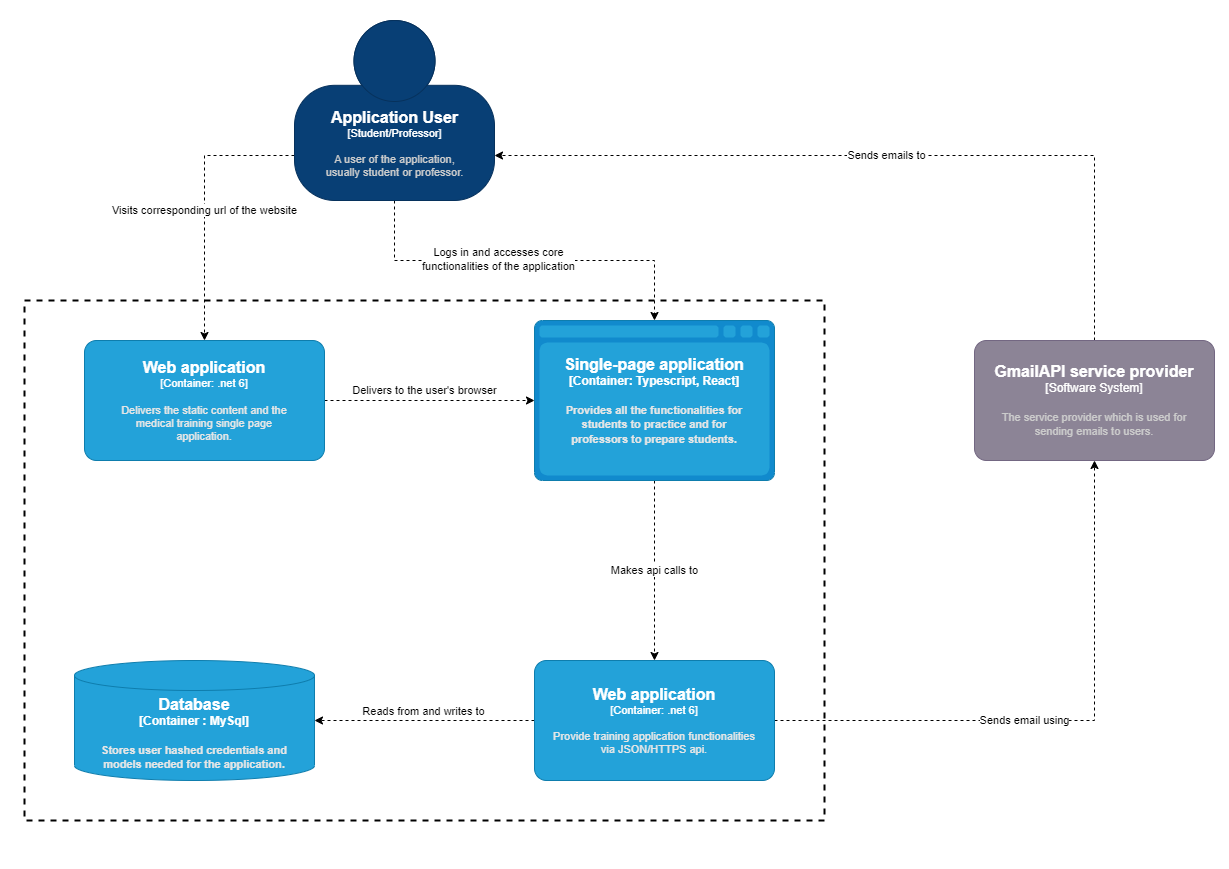
\includegraphics[width=\textwidth,height=\textheight,keepaspectratio]{img/c4_level2.png}
    \caption{Level 2 C4 model}
\end{figure}

The second level of the C4 model provides a more detailed view of the system architecture, focusing on the relationships and responsibilities of the various components within the system. The system consists of four main components: the application users, the web application, the backend, and the Gmail API service provider.

The application users are students and professors who interact with the system through the web application. When they visit the URL of the web application, it delivers the necessary content and a single page application (SPA). The SPA is a client-side application that runs in the user's web browser and provides the interface through which the application users can access the core functionality of the system.

The web application is responsible for serving the SPA to the application users and handling their interactions with it. When the application users perform an action within the SPA, such as logging in or accessing a group, the SPA makes an API call to the backend to request the necessary data or to perform the desired action.

The backend is a separate component that handles most of the processes within the system. It is responsible for reading and writing data to and from the database, as well as processing the API requests made by the SPA. It is also responsible for communicating with the Gmail API service provider, which is used to send emails to the application users.

The Gmail API service provider is a third-party component that is integrated into the system to provide email functionality. It is used specifically to send emails to the application users, such as when they register for an account.

Overall, the second level of the C4 model for this system describes the relationships and responsibilities of the various components within the system. The application users interact with the web application and SPA to access the core functionality of the system, and the web application communicates with the backend to retrieve data and perform actions. The backend, in turn, communicates with the Gmail API service provider to send emails when necessary.

\section{Client applications}

\subsection{Programming language}
\subsubsection{Typescript}
\begin{enumerate}
    \item One of the reasons why Typescript was chosen over Javascript is that Typescript is strongly typed \cite{typescriptDocs}, whereas Javascript is not, this difference makes it easier to know which part of the code is causing the problem. To put it simply, Typescript is much safer.
    \item TypeScript helps you catch and fix errors before you run your code, making it easier to spot and fix bugs.
    \item TypeScript makes it easier to refactor your code, as the type system helps you understand how different parts of your code are related and how they are used.
    \item As Typescript is, in layman’s terms, a typed Javascript, it has a large and active community of users and developers, providing a wealth of resources and support for those working with the language.
    \item TypeScript has excellent documentation and a large number of resources available, making it easy to learn and use.
    \item TypeScript has strong support for object-oriented programming concepts, such as classes, interfaces, and inheritance, making it a good choice for projects that need to use these features.
\end{enumerate}

\subsection{Libraries/Frameworks}

\subsubsection{React}

\begin{enumerate}
    \item Rather than going for a mobile or desktop app, the need for the application to be web-based is rather important for this project as the intended users will most likely find it more convenient to access the app via a web browser. Therefore, in this project, we decided to use the React library.
    \item React was our choice for this project because using vanilla Javascript would be downright nonsensical. In comparison to Angular and Vue, React is rather easier to pick up, which is quite important as this allows the team to learn the library with relative ease and start creating complex web applications.
    \item React has a large and active community of users and developers, providing a wealth of resources and support for those working with the library.
    \item React is relatively sophisticated, with a virtual DOM that allows for dynamic rendering and quick updates to the user interface, making the application very reactive \cite{reactDocs}.
    \item React has strong support for reusable components, making it easy to build and maintain large and complex applications. Having reusable components means that developers can reduce boilerplate code by creating components that are abstract and thereby applicable to many places in the code.
\end{enumerate}

\subsubsection{i18next}
\begin{enumerate}
    \item The university, for which this app is designed, has both Polish-speaking students and English-speaking students, so there is a need to localize the app. The i18next library provides tools which make localization simpler than it needs to be.
    \item i18next has a large and active community of users and developers, providing lots of resources and support for those working with the library.
    \item i18next is highly configurable, allowing you to customize how it handles translations and language detection, meaning users using English as their default language on browsers will automatically see English translations \cite{i18nextDocs}.
    \item i18next is lightweight and efficient, with a small footprint that won't add unnecessary bloat to the project.
    \item i18next supports a wide range of platforms and frameworks, including web, mobile, and server-side applications. For our application it was simpler to store the translations on the frontend and i18next does provide such a feature.
    \item There are many other localization libraries for example React-Intl, however, given the fact that we have experience in i18next, we decided to stick with it.
\end{enumerate}

\subsubsection{React query (tanstack query)}

\begin{enumerate}
    \item React query takes away much of the boilerplate code that is required when writing fetch requests for API. There are many functionalities, which when used with QueryClient, makes updating and removing data on the page as simple as calling a single function.
    \item React Query is a lightweight and efficient library for fetching, caching, and updating data in React applications. \cite{tanstackQueryDocs}
    \item React Query has a simple and intuitive API that makes it easy to use and integrate into our project, letting us focus on sending requests to the backend as opposed to building our own API.
    \item React Query has built-in support for handling common data fetching tasks, such as pagination, filtering, and sorting, making it a good choice for projects that need to work with large or complex data sets.
    \item React Query has a flexible and configurable caching system that allows you to control how data is fetched and stored, making it a good choice for projects that need to optimize performance or manage data efficiently.
    \item React Query has a large and active community of users and developers, providing a wealth of resources and support for those working with the library.
    \item React Query is lightweight and efficient, with a small footprint that won't add unnecessary bloat to the project.
    \item React Query has a built-in dev-tool which helps us ensure that the requests are in fact being called and the data that is received is indeed the correct data that is being called for.
\end{enumerate}

\subsubsection{React-chartjs}
\begin{enumerate}
    \item React Chart.js is a relatively customizable library, allowing developers to create charts that fit the specific needs and design of their application. This means, it helps us to focus on passing in the data into the React component rather than build everything from scratch.
    \item It is easy to use and integrate into a React project, with a simple API and numerous pre-built components. In reference to the previous point, Chart.js is not as customizable as say D3js but that is why it is chosen because in D3js you have to define charts yourself from ground up.
    \item It has a wide range of chart types available, including bar charts, line charts, pie charts, and more. \cite{chartjs} Given the purpose of our project it was important to have multiple options to see which fits best for the given component we want to use Chart.js in.
\end{enumerate}

\subsubsection{Material UI}

\section{Backend applications}
\subsection{Programming language}
\subsubsection{C\#}
\begin{enumerate}
    \item The greatest reason for the choice of C\# over other languages is the fact that every member has had experience creating full stack applications with C\# before.
    \item C\# has a big community, meaning there is lots of resource to refer to.
    \item On top of that, C\# is a statically-typed language, which means that it catches errors at compile-time rather than runtime. This can lead to more stable and reliable code. \cite{csharpDcos}
    \item C\# also has strong support for test-driven development, which can help ensure that our code is not full of bugs and easy to maintain.
\end{enumerate}
\subsection{Libraries/Frameworks}
\subsubsection{ASP.NET}
\begin{enumerate}
    \item ASP.NET is the framework chosen to be used for this application. There are many advantages to ASP.NET, it is cross-platform, and standardized but it is first and foremost an open-source framework.
    \item ASP.NET is a competitor with many other frameworks such as spring, Django, PHP laravel and nodejs express to name a few. While other frameworks do the job, the majority of the team member has experience with C\#.
    \item Strong support and a large community, ASP.NET is a mature, widely-used web development framework with a strong developer community and good documentation and resources which is extremely useful for creating an app. \cite{aspnetDocs}
    \item ASP.NET has many built-in features and tools that help increase productivity and speed up the development process.
    \item ASP.NET has a number of built-in security features, such as validation and encryption, to help protect web applications and keep data safe.
\end{enumerate}

\subsubsection{EntityFrameworkCore (EFC)}
\begin{enumerate}
    \item Entity Framework Core is a lightweight, extendable, open source, cross-platform version of the well-maintained Entity Framework data access technology. \cite{efcoreDocs}
    \item In comparison to Dapper, a micro ORM alternative to EFC, EFC offers an abstraction from SQL, allowing developers to focus on writing code in C\#.
    \item Furthermore, developing with Dapper requires more time because the reason for choosing Dapper is typically to write your own SQL as opposed to EFC where SQL are optimized under the hood.
\end{enumerate}
\subsubsection{Pomelo EntityFrameworkCore MySql}
\begin{enumerate}
    \item The reason for the use of Pomelo EFC is simply due to the fact that there seems to be no alternative as of the time of choosing it. While there are other similar alternatives, for example Npgsql, but it is used with a difference database and that is a topic to be discussed later.
    \item Pomelo EFC does not replace EFC completely, it only extends it as a provider for databases that are compatible with MySql, having this Object-relational mapping (ORM) helps us to connect object code to a MySql database.
\end{enumerate}

\subsubsection{Gmail API}
\begin{enumerate}
    \item The Gmail API has built-in support for OAuth 2.0 authentication, which makes it easier to securely authenticate users and access their data. \cite{gmailapiDocs}
    \item The Gmail API is free to use for the first 15 GB of data transferred per month, which should be sufficient for most small to medium-sized applications.
    \item Gmail API was chosen over SendGrid mainly because there was reason to choose it. Given the scale of the application and how the only usage of email is for registration and resetting password, the final decision was Gmail API.
\end{enumerate}

\section{Persistence layer}
\subsection{Database}

\subsubsection{MySql}
\begin{enumerate}
    \item MySql is a good database choice as the purpose of our application is to be used internally for a school so it was in the school’s and our best interest to keep things simple and as cheap as possible. Therefore, an open-source database \cite{mysqlDocs} was the one we chose as it is a cost-effective choice.
    \item MySQL has a long history and has been widely adopted by many organizations, making it a tried and tested choice for the project, among other benefits.
    \item MySQL supports a wide range of data types and data storage options, including support for large volumes of data and support for different storage engines.
    \item While Microsoft SQL (MSSQL) server  may have been the more "obvious choice" considering the tech stack of this project but due to the fact that MSSQL is not open-sounrce, it was not chosen. 
\end{enumerate}

\section{Codebase showcase}

\subsection{Frontend}

\subsubsection{API requests}

The most important part of the frontend is arguably the API requests. Wihtout Application programming interface (API) requests there is no way to get data from the backend, rendering the frontend essentially pointless. Therefore, it is important that these functions that handle API requests work properly. 

The project is a CREATE, READ, UP-DATE and DELETE (CRUD) application that is built with the representational state transfer (RESTful) API architectural style in mind. Often times, the end points will need to have payload that are relatively complex, therefore it is usually delivered in JSON format. On top of that, because OAuth2 is used in this project as a security measure, every request that requires validation must send a token \cite{oauthSimplified}, in this case JSON web token (JWT). \cite{restfulOReilly}

\vspace{0.1cm}

\begin{lstlisting}
    const baseFetch = async (path: string, method: string, jwt: string): Promise<Response> => {
  return await fetch(`${apiPath.BASE_URL}${path}`, {
    method: method,
    headers: {
      "Access-Control-Allow-Credentials": "true",
      Authorization: `Bearer ${jwt}`,
      "Content-Type": "application/json",
    },
  });
};
const baseFetchWtihPayload = async (path: string, method: string, jwt: string, payload: string): Promise<Response> => {
  return await fetch(`${apiPath.BASE_URL}${path}`, {
    method: method,
    body: payload,
    headers: {
      "Access-Control-Allow-Credentials": "true",
      Authorization: `Bearer ${jwt}`,
      "Content-Type": "application/json",
    },
  });
};
\end{lstlisting}

The two functions {\bfseries baseFetch} and {\bfseries baseFetchWithPayload} above are core components of the frontend for API requests. Most API requests that require data from the database or makes changes to the database will use one of these two functions by given the required parameters, along with the JWT in side the Aurtorization header.

\subsubsection{ReactQuery Hooks}

One of the more important part of the frontend is arguably the hooks that take care of API requests. While they do not look like the most complex code out of the entire codebase, the functionalities they provide and the code under the hood is extremely sophisticated.

Let's have a look at the landing page - Dashboard.
\begin{figure}[H]
    \centering
    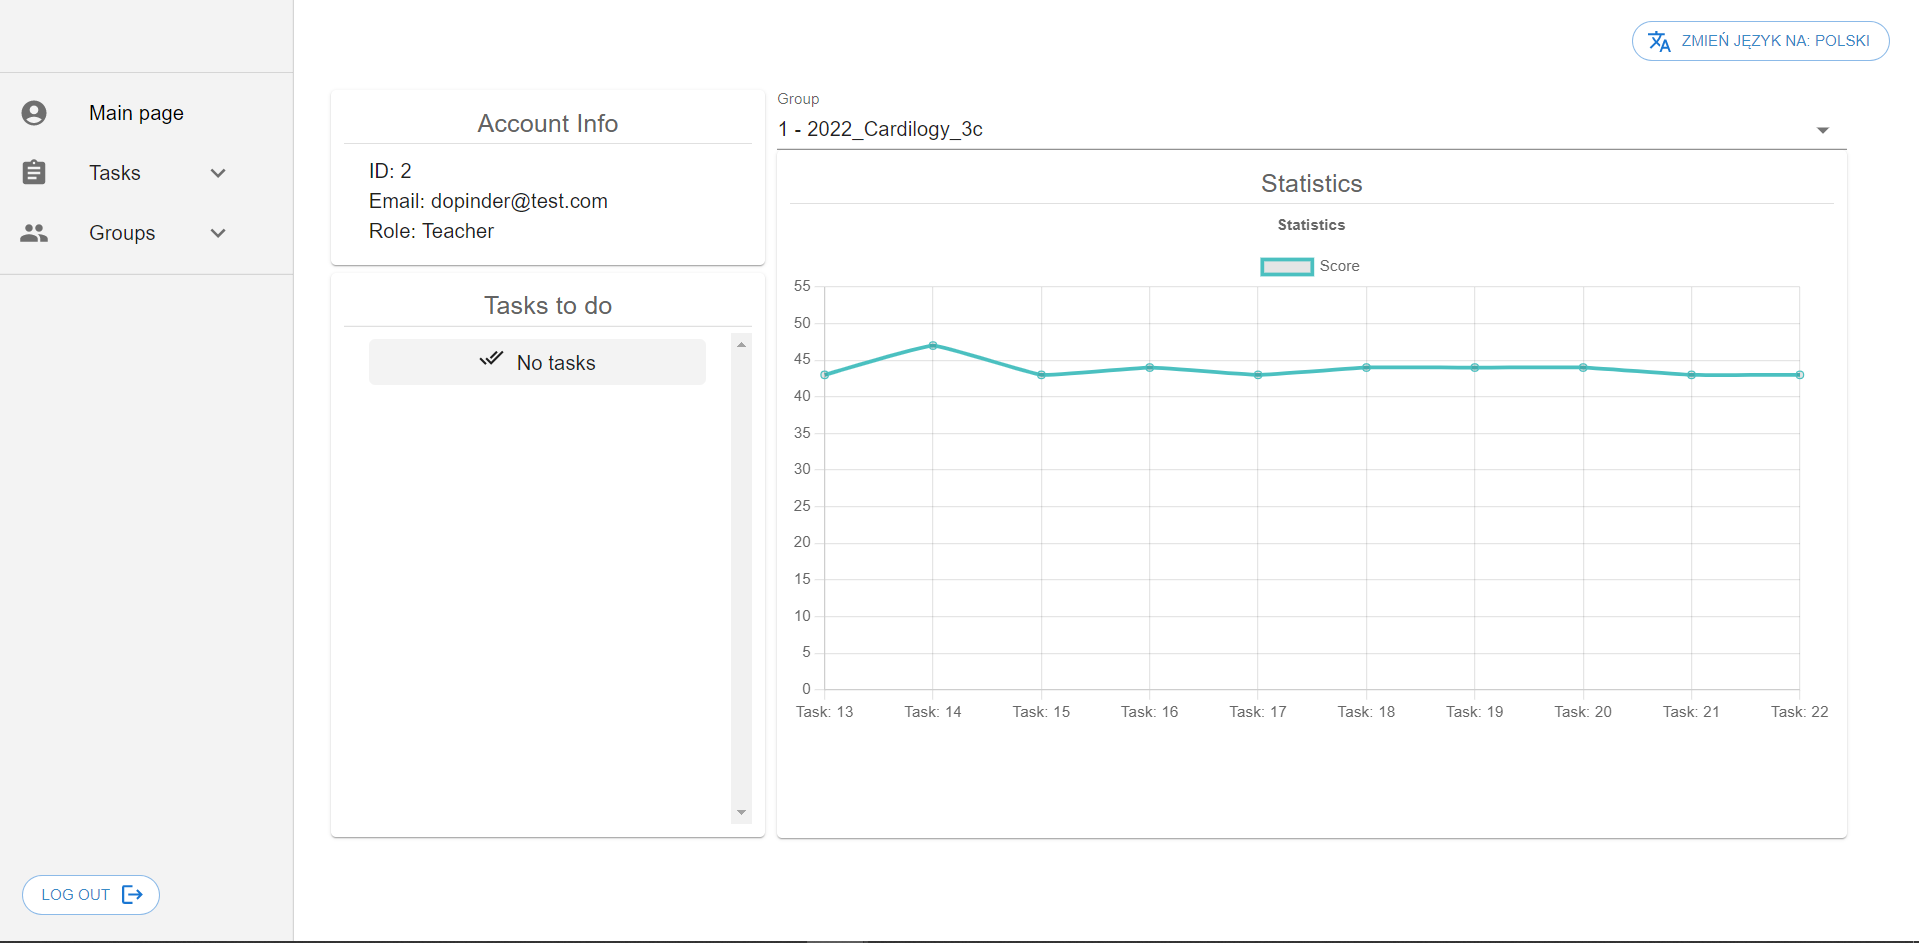
\includegraphics[width=\textwidth,height=\textheight,keepaspectratio]{img/dashboardPage.png}
    \caption{Dashboard}
\end{figure}
\pagebreak

The dashboard is divided into essentially three main parts, UserDetailCard, TodoTasksCard and UserStatsCard. UserDetailCard shows the information about the user's account (ID, Email, Role). TodoTasksCard shows tasks that haven't been done yet. And most importantly the UserStatsCard provides a line chart that shows the score of every task for a given group.

\vspace{0.5cm}
\begin{lstlisting}
const Dashboard = () => {
  return (
    <div style={{ display: "flex" }}>
      <Grid item xs={5} style={{ width: "28%" }}>
        <div style={{ width: "100%", height: "20%" }}>
          <UserDetailCard style={{ marginBottom: "20px" }} />
        </div>
        <div style={{ width: "100%", height: "70%" }}>
          <TodoTasksCard style={{ marginBottom: "20px" }} />
        </div>
      </Grid>
      <Grid item xs={10} style={{ width: "69%", marginLeft:'10px' }}>
        <div style={{ width: "100%", height: "100%" }}>
          <UserStatsCard />
        </div>
      </Grid>
    </div>
  );
};
\end{lstlisting}

Each component inside Dashboard makes an API request to retrieve the necessary data and they do it with the help of custom hooks that use React Query.\\
\\
UserDetailCard uses the following hook:
\begin{lstlisting}
    const { userData, userLoading, userIsError } = useUserDetailQuery();
\end{lstlisting}
TodoTasksCard uses the following hook:
\begin{lstlisting}
    const { tasks, tasksLoading, tasksIsError } = useGetTasks();
\end{lstlisting}
\pagebreak
UserStatsCard uses the following hooks:
\begin{lstlisting}
    const { finishedTasks, finishedTasksInfoLoading, finishedTasksIsError, finishedTasksRefetch } = useGetFinishedTasksByGroup(selectedGroup);

    const { group, groupInfoLoading, groupIsError, groupIsFetching } = useGetCurrentGroups();
\end{lstlisting}

Having a look at an example, say {\bfseries useUserDetailQuery}, if we go deeper and look at what this hook does, you will notice that it is calling another function with useQuery. The function within useQuery utilizes the previously mentioned {\bfseries baseFetch} to fetch the details about the account that called the corresponding endpoint.

\begin{lstlisting}
    export const useUserDetailQuery = () => {
      const {
        data: userData,
        isError: userIsError,
        isLoading: userLoading,
        error: userError,
      } = useQuery("dashboard", async (): Promise<IUserDTO> => {
        const user = await getDashboard();
        return user;
      });
    return { userData, userIsError, userLoading, userError };
    };
\end{lstlisting}

\subsubsection{ReactQuery features}

One of the most important ReactQuery component is the QueryClient, it provides many methods that can be used to fetch and cache a query, all of which provide a different purpose and method of querying.

\begin{lstlisting}
    const queryClient = new QueryClient({
      defaultOptions: {
        queries: {
          refetchOnWindowFocus: false,
          retry: 3,
          retryDelay: 3000,
        },
      },
    });
\end{lstlisting}

One of the methods from QueryClient is {\bfseries refetchQueries}, it accepts a string argument {\bfseries queryKey} which is used to select the correct query for making the API request. To be more specific, {\bfseries useUserDetailQuery} has queryKey "dashboard", meaning if there is a need to refresh the data, you need only to call the refetchQueries function and pass "dashboard" as its argument.

You may have noticed that in the useUserDetailQuery snippet, {\bfseries useQuery} was called within the hook. The useQuery hook is the most basic feature of ReactQuery and it is primarily used for reading data. From the useQuery hook you may receive the data itself, boolean value of whether it is loading, whether there was an error and more.

However, let's say that we would like to remove data, say from a list, then we cannot use useQuery. The reason for that is due to the fact that useQuery is first and foremost used for read only, not writing. In order to modify data we must use another helpful hook called {\bfseries useMutation}

\begin{lstlisting}
    const removeTaskGroupMutation: UseMutationResult<void, Error, RemoveParamMutate> = useMutation<void, Error, RemoveParamMutate>(async ({ taskId, groupId }) => {
    await removeTask(taskId, groupId);
    await queryClient.invalidateQueries("tasksInfoByGroup");
  });
\end{lstlisting}

In this code snippet, the useMutation hook makes an API request removeTask to remove a task that was assigned to the corresponding group, then it invalidates the query with a queryKey "tasksInfoByGroup"; this queryKey comes from another hook that was used to first fetch a list of tasks.

\pagebreak
\subsection{Backend}

\subsubsection{Setting up Pomelo EFC}

One of the most crucial part of the project is to set up the database driver in order to use the ORM. Thankfully, this can be done very easily by using AddDbContext after installing the Pomelo EFC package. 

\begin{lstlisting}
    builder.Services.AddDbContext<ApplicationDbContext>(dbContextOptions =>
    dbContextOptions.UseMySql(cs,
            ServerVersion.AutoDetect(cs)
            )
    )
\end{lstlisting}

Once we have set up the database driver we may start using it. We can then inject dependencies, in this case the Service classes which we will use for our Controllers when we receive API request on an endpoint.

\begin{lstlisting}
    .AddScoped<IUserService, UserService>()
    .AddScoped<IGroupService, GroupService>()
    .AddScoped<IUserGroupService, UserGroupService>()
    .AddScoped<ITaskService, TaskService>()
    .AddScoped<IJwtTokenService, JwtTokenService>()
    .AddScoped<IEmailService, EmailServices>()
\end{lstlisting}

By injecting dependencies, it makes the component more modular and easier to test, since they are passed in from the outside rather than being hard-coded and makes the code overall easier to maintain. This software design patterns allows us to achieve the Inversion of Control (IOC) between classes and their dependencies. \cite{dotnetDocs}

\pagebreak
\subsubsection{Authentication}

In the following section we are setting up token validation for the application. This enables us to authenticate users that are sending requests to endpoints. In ASP.NET, authentication works in such a way that service IAuthenticationService is used by authentication middleware. The authentication service processes any authentication related actions and thereby giving us security OAuth measure over the internet.

\begin{lstlisting}
    builder.Services.AddAuthentication(JwtBearerDefaults.AuthenticationScheme).AddJwtBearer(options =>
{
    options.TokenValidationParameters = new TokenValidationParameters()
    {
        ValidateIssuer = true,
        ValidateAudience = true,
        ValidateLifetime = true,
        ValidateIssuerSigningKey = true,
        ValidAudience = configuration["JWT:ValidAudience"],
        ValidIssuer = configuration["JWT:ValidIssuer"],
        IssuerSigningKey = new SymmetricSecurityKey(Encoding.UTF8.GetBytes(configuration["JWT:Secret"])),
        ClockSkew = TimeSpan.Zero
    };
});
\end{lstlisting}

After setting up authentication for our application, every request that is trying to access restricted resource must come from authorized users. By providing claims, the application is now able to grant authorization based on whether it is valid or not.

\pagebreak

\subsubsection{Gmail API}

In order to use this application one must first create an account by going through the registration process, unless of course they have an account already. To achieve this, we need to use email activation. Certainly, we need not to go through the email activation process, however, the purpose of it is to verify the user and to ensure that this email is real. The difference between an active and a non-existent email is, naturally. the fact that non-existent emails cannot activate accounts. As for inactive emails, we do not need to worry because they may or may not be activated.

From the perspective of the application we only need to make sure those accounts that have had a link with activation token sent to their email to be properly activated after visiting the URL. In order to achieve this, we must first set up an email service, in this application, Gmail API was the service of choice.

To make Gmail API work we need to complete the following steps as provided on Google's guide \cite{gmailApiAuthDocs}:

    \begin{enumerate}
    \item The application must be registered in the Google API console.
    \item Users must grant explicit access permission for the app when the app launches for the first time.
    \item Assuming the user agrees, the application will request for credential to access the Gmail API.
    \item Refresh the credentials (if necessary).
\end{enumerate}

Naturally, we need a Gmail account to register our application in the Google API console. Once we have registered our application, we need to create an OAuth client ID because Gmail API does not use Simple Mail Transfer Protocol (SMTP). Gmail API is a RESTful API that can be used with any programming language that can make HTTP requests and parse JSON responses, it achieves this by using OAuth 2.0 protocol for authorization and authentication.

Once we have created our OAuth client ID, we can download it as JSON file and use it in our application. In the following code snippet, we have a function that is used for sending emails with EmtailTemplate being the source of destination address, subject and body of our email. Notice we are reading from the file "client\_secret.json", this is the OAuth client ID we have downloaded from the Google API console, inside it we can find all the relevant credentials.

Notice that we have a string of array called Scopes. Gmail API allows developers to specify Auth Scopes, the reason for this is to grant as little permission as possible to a user at a given time because some scopes may be used for restricted resources. \cite{gmailapiDocs} In this application, we only need to use the "https://www.googleapis.com/auth/gmail.send" scope, which is GmailSend in the code below.

\begin{lstlisting}
    public Task<bool> SendEmail(EmailTemplate data)
    {
        try
        {
            string[] Scopes = { GmailService.Scope.GmailSend };
            UserCredential credential;
            using (var stream = new FileStream(
                "./client_secret.json",
                FileMode.Open,
                FileAccess.Read
            ))
\end{lstlisting}

Next, we prepare the credentials we need to allow our app to verify with a Google account. With our credentials prepared, we can not create our Gmail API service. Notice that we are creating a folder called "token\_Send.json", this folder will save, among other important data, the access token and refresh token for the application to use every time it accesses Gmail API.

\begin{lstlisting}
    {
        string credPath = "token_Send.json";
        credential = await GoogleWebAuthorizationBroker.AuthorizeAsync(
                     GoogleClientSecrets.FromStream(stream).Secrets,
                      Scopes,
                      "user",
                      CancellationToken.None,
                      new FileDataStore(credPath, true));
    }
    // Create Gmail API service.
    var service = new GmailService(new BaseClientService.Initializer()
    {
        HttpClientInitializer = credential,
        ApplicationName = "ecg",
    });
\end{lstlisting}

Lastly, we simply create the message we want to send with the proper headers and send our account activation token or perhaps reset password token depending on which endpoint the user was calling.

\begin{lstlisting}
     string message = $"To: {data.EmailTo}\r\nSubject: {data.EmailSubject}\r\nContent-Type: text/plain;charset=utf-8\r\n\r\n{data.EmailBody}";
    var newMsg = new Google.Apis.Gmail.v1.Data.Message();
    newMsg.Raw = this.Base64UrlEncode(message.ToString());
    Message response = await service.Users.Messages.Send(newMsg, "me").ExecuteAsync();
\end{lstlisting}

\pagebreak

\subsubsection{Login endpoint}

Up to this point we have been looking at how things are set up for this project, let us look at the most basic and perhaps most crucial endpoint for this project, the Login endpoint.

In order for our users to login to use our application they must send a request to the URL "/Auth/Login" with the payload "UserLoginDTO" which consists of the user's email and password.

\begin{lstlisting}
    [HttpPost(ApiRoutes.Auth.Login)]
    public async Task<IActionResult> Login(UserLoginDTO request)
\end{lstlisting}

We first and foremost check for whether there exists a user with such an email because if there is not such email, this most likely means the user has not registered yet. Then we check whether the account is activated, activating account is important because theoretically anybody is able to access our website, and we do not want that. The purpose of only allowing accounts that have been activated is so that only users with an email from the medical university's domain may login.

\begin{lstlisting}
    if (!await _service.ExistsUserByEmailAsync(request.Email))
    {
        return StatusCode(401);
    }

    if (!await _service.AccountActivated(request.Email))
    {
        return StatusCode(401);
    }
\end{lstlisting}

Next, we check whether the password submitted by the user matches the given email. In order to do this, we will need the submitted password, the hash and the salt in order to compute the correct value. If the value computed checks out, this means our user gave the correct password. Note that passwords are not stored in plain texts whatsoever because doing so is a risk of security, the preferred way is to compute the hash and compare them.

\begin{lstlisting}
    var hash = await _service.GetUserHash(request.Email);
    var salt = await _service.GetUserSalt(request.Email);
    if (hash == null || salt == null)
    {
        return StatusCode(401);
    }
    if (!_service.VerifyPasswordHash(request.Password, hash, salt))
    {
        return StatusCode(401);
    }
\end{lstlisting}

Finally, once all the previous checks have passed, we need only to provide the user its data in order persist information on the client side, and JWT so that every consequent API requests made to access restricted resources will bear it in the Hypertext Transfer Protocol (HTTP) header, thereby allowing us to authenticate and authorize the user.

\begin{lstlisting}
    JwtTokenDTO? jwt = await _service.RenewAccessRefreshToken(request.Email);
    if (jwt == null)
    {
        return StatusCode(500);
    }
    UserDTO? userData = await _service.GetUserByEmailReturnDTO(request.Email);
    if (userData == null)
    {
        return StatusCode(500);
    }
    return Ok(new LoginResponseDataDTO
    {
        UserData = userData,
        JwtToken = jwt
    });
\end{lstlisting}

\pagebreak

\section{Testing and deployment}

\subsection{Unit Tests}
For the Unit Tests it was decided to use \textbf{XUnit} and \textbf{Moq}.
\begin{figure}[H]
    \centering
    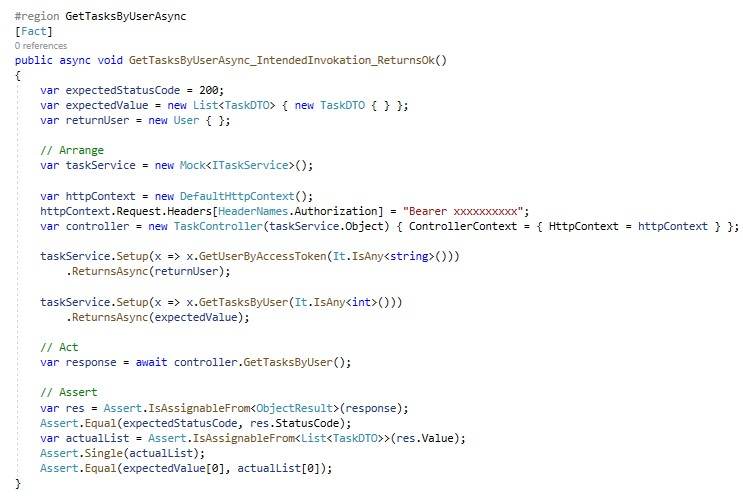
\includegraphics[width=\textwidth,height=\textheight,keepaspectratio]{img/TestExample.jpg}
    \caption{Example of test for GetTasksByUserAsync()}
\end{figure}

\section{Documentation for the users}

\subsection{Main pages before login}

\subsubsection{Login page}
Login page will be the main page of the application. From here, you are able to login, go to Registration page or Reset password page.

\subsubsection{Register page}
In the registration page, you are able register a new account. Once you have sent a request to the server for registering an account, you will receive an email with an activation link. By opening the activation link you received, you will be directed to the activation page. Here, the system will automatically activate your account and once it is activated you will be redirected back to the login page where you may login.

\subsubsection{Reset password page}
The reset password page is where you can reset your password in the event that you forget your password. Similar to the registration page, once you have filled in the form you will receive an email with a link that takes you to a page where you may enter your new password.

\pagebreak

\subsection{Pages after login}

\subsubsection{Page layout}
After login, you will notice a sidebar where you can navigate through all the pages. In the bottom left you will find the logout button which logs you out if you click on it. Lastly, in the top right, you may find a button for switching the translation of the page to either Polish or English.

\subsubsection{Landing page - Dashboard}
The landing page, meaning the page you enter after login, will be the dashboard. On this page, you will be able to see your account detail, tasks to be done and statistics of your tasks within the group you have selected.

\subsubsection{Task section}

Within the task section, found on the sidebar, you will notice two subsections, namely "Tasks to do" and "Task History".

\begin{enumerate}
    \item Tasks to do

    Within Tasks to do, you will be able to see all the tasks that are waiting for you to complete, if there is any. Clicking on "Start task" will bring you to the next page where you will begin solving a task. While solving a task, you will be able to view or hide ecg diagram and once you have filled in your answer or even if you did not, you may submit your task. After submitting, you will enter the summary page in which you will received details about a certain illness.

    \item Task History

    As the name suggest, inside task history, you will be able to choose a task to view your choices. Inside a chosen task, you will see all the questions and answers. There are three types of color coding. Green - the answer and your choice matched. Yellow - the answer should have been marked but was not. Red - the choice was incorrect and was not supposed to be marked.
    
\end{enumerate}

\subsubsection{Group section}
Within the group section, you will find two subsections, "Groups" and "Group management". If you are a student you will see only "Groups".

\begin{enumerate}
    \item Groups

    Inside Groups, you will see all the groups you belong in. You may also enter a group by providing a group code below. Once you submit a group code, you will be automatically added to this group, assuming the code you gave was correct.
    
    \item Group management

    Inside the Group management section, teachers will be able to see only the groups which they have created. You may remove a group by clicking the remove button or add a new group by providing a name for your group and clicking the create group button below.

    If you instead click on details button of a group, you will be directed to the group's detail page. Here you will be able to see every user that joined this group and group code. You can remove a user from the group or if you instead click on details you can view this user's details and statistics, similar to the dashboard page.

    You will also notice "Check assigned tasks" button in the group details page. Clicking on checked assigned tasks button will take you to another page where you can see all the tasks you have assigned. Here you will be able to add new tasks or remove one.
    
\end{enumerate}

\pagebreak
% contribution in the end
\section{Contribution}
\begin{tabular}{ |p{4cm}|p{9cm}|  }
\hline
\bf{Author}& \bf{Implementation} \\
\hline
Somebody& Something\\ 
\hline
\end{tabular}

\pagebreak
\printbibliography

\end{document}
